%Talk given virtually for SIAM UQ 2020 March
\documentclass[10pt,compress,xcolor={usenames,dvipsnames},aspectratio=169]{beamer}
%\documentclass[xcolor={usenames,dvipsnames},aspectratio=169]{beamer} %slides and 
%notes
\usepackage{amsmath,
	amssymb,
	datetime,
	mathtools,
	bbm,
	%mathabx,
	array,
	booktabs,
	xspace,
	multirow,
	calc,
	colortbl,
	siunitx,
 	graphicx}
\usepackage[usenames]{xcolor}
\usepackage[giveninits=false,backend=biber,style=nature, maxcitenames =10, mincitenames=9]{biblatex}
\addbibresource{FJHown23.bib}
\addbibresource{FJH23.bib}
\usepackage{newpxtext}
\usepackage[euler-digits,euler-hat-accent]{eulervm}
\usepackage{media9}
\usepackage[autolinebreaks]{mcode}
\usepackage[tikz]{mdframed}


\usetheme{FJHSlimNoFoot169}
\setlength{\parskip}{2ex}
\setlength{\arraycolsep}{0.5ex}

%\renewcommand{\qedsymbol}{}

\DeclareMathOperator{\sol}{SOL}
\DeclareMathOperator{\app}{APP}
\DeclareMathOperator{\alg}{ALG}
\DeclareMathOperator{\ACQ}{ACQ}
\DeclareMathOperator{\ERR}{ERR}
\DeclareMathOperator{\COST}{COST}
\DeclareMathOperator{\COMP}{COMP}
\DeclareMathOperator{\LIN}{LINEAR}
\DeclareMathOperator{\BAD}{BAD}
\newcommand{\dataN}{\bigl(\hf(\vk_i)\bigr)_{i=1}^n}
\newcommand{\dataNj}{\bigl(\hf(\vk_i)\bigr)_{i=1}^{n_j}}
\newcommand{\dataNjd}{\bigl(\hf(\vk_i)\bigr)_{i=1}^{n_{j^\dagger}}}
\newcommand{\ERRN}{\ERR\bigl(\dataN,n\bigr)}

\newcommand{\Sapp}{S_{\textup{app}}}
\newcommand{\LambdaStd}{\Lambda^{\textup{std}}}
\newcommand{\LambdaSer}{\Lambda^{\textup{ser}}}
\newcommand{\LambdaAll}{\Lambda^{\textup{all}}}
\newcommand{\oton}{1\!:\!n}
\newcommand{\talert}[1]{\alert{\text{#1}}}
\DeclareMathOperator{\init}{init}
\DeclareMathOperator{\GP}{\cg\cp}
\newcommand{\MLE}{\textup{EB}}
\newcommand{\mCtheta}{{\mathsf{C}_{\vtheta}}}
\newcommand{\mCInv}{\mathsf{C}^{-1}}
\newcommand{\tvg}{\widetilde{\vg}}

%\DeclareMathOperator{\app}{app}

\providecommand{\HickernellFJ}{H.\xspace}


\iffalse

\fi

\renewcommand{\OffTitleLength}{-7ex}
\setlength{\FJHThankYouMessageOffset}{-8ex}
\title{The Reisz Representation Theorem}
\author[]{Fred J. Hickernell}
\institute{Department of Applied Mathematics \&
	Center for Interdisciplinary Scientific Computation \\  Illinois Institute of Technology \quad
	\href{mailto:hickernell@iit.edu}{\url{hickernell@iit.edu}} \quad
	\href{http://mypages.iit.edu/~hickernell}{\url{mypages.iit.edu/~hickernell}}}

\thanksnote{Thanks to the Illinois Tech Student Chapter for the invitation}
	
\event{My Favorite Theorem}
\date[]{???, 2021}

\input FJHDef.tex


\newlength{\figwidth}
\setlength{\figwidth}{0.25\textwidth}

\newlength{\figwidthSmall}
\setlength{\figwidthSmall}{0.2\textwidth}

\newcommand{\financePict}{\href{http://i2.cdn.turner.com/money/dam/assets/130611131918-chicago-board-options-exchange-1024x576.jpg}{\includegraphics[width
		= 3cm]{ProgramsImages/130611131918-chicago-board-options-exchange-1024x576.jpg}}}
	
	\newcommand{\scoop}[1]{\parbox{#1}{
\includegraphics[width=#1]{IceCreamScoop.eps}}\xspace}
	\newcommand{\smallscoop}{\scoop{1cm}}
	\newcommand{\medscoop}{\scoop{1.8cm}}
	\newcommand{\largescoop}{\scoop{3cm}}
	\newcommand{\ICcone}[1]{\parbox{#1}{
\includegraphics[width=#1,angle=270]{MediumWaffleCone.eps}}\xspace}
	\newcommand{\medcone}{\ICcone{1.2cm}}
	\newcommand{\largercone}{\parbox{2.2cm}{\vspace*{-0.2cm}
\includegraphics[width=1cm,angle=270]{MediumWaffleCone.eps}}\xspace}
	\newcommand{\largecone}{\ICcone{1.8cm}}
	\newcommand{\smallcone}{\parbox{1.1cm}{
\includegraphics[width=0.5cm,angle=270]{MediumWaffleCone.eps}}\xspace}

	

\newcommand{\northeaststuff}[3]{
	\begin{tikzpicture}[remember picture, overlay]
	\node [shift={(-#1 cm,-#2 cm)}]  at (current page.north east){#3};
	\end{tikzpicture}}


\begin{document}
	\tikzstyle{every picture}+=[remember picture]
	\everymath{\displaystyle}

\frame{\titlepage}


\section{Background}

\begin{frame}{Main Idea}
    What seems \alert{obvious} for $d$-dimensional vectors becomes a power tool for \alert{numerical analysis}
    
    \begin{description}
    \item[Obvious]<2-> If $\LIN: \reals^3 \to \reals$ is any \alert{linear, real-valued} function, \uncover<2-4>{meaning,
    \[
    \LIN(c\vf + \vh) = c \LIN(\vf) + \LIN(\vh) \qquad \forall \vf, \vh \in \reals^3, \ c \in \reals,
    \]}
    then we can represent $\LIN(f)$ as an \alert{inner product}\uncover<2-4>{:
    \[
    \LIN(\vf) = g_1 f_1 + g_2 f_2 + g_3 f_3 = \vg^T \vf =: \ip{\vg}{\vf} \equiv \vg \bigcdot \vf \quad \forall \vf \in \reals^3, \text{ where $\vg \in \reals^3$ is fixed}.
    \]
    \only<2>{The vector $\vg$ corresponds to the \alert{coefficients}.}}
   \item[Powerful Tool]<3-> Generalization allows us to derive \alert{error bounds} for numerical algorithms, e.g.,
   \[
   \biggl\lvert\only<4->{\underbrace}{\int_{[0,1]^d} f(\vx) \, \dif \vx}\only<4->{_{\substack{\text{\alert{average} of $f$} \\ \text{e.g., option price}}} \quad}  - \only<4->{\underbrace}{\frac 1n \sum_{i=1}^n f(\vx_i)}\only<4->{_{\substack{\text{\alert{average} of $f$ values} \\ \text{e.g., payoffs under various scenarios} }}} \biggr\rvert \le \only<5->{\underbrace}{\BAD(\vx_1, \ldots, \vx_n)}\only<5->{_{\Large\substack{\alert{\text{Concentrate on }} \\
   \alert{\text{choosing the $\vx_i$ well}}}}} \, \BAD(\vf)
   \]
    \end{description}
\end{frame}

\section{Riesz Rep Theorem in $\reals^d$}

\begin{frame}{Riesz Representation Theorem for $\reals^3$}
\begin{theorem}
    If $\LIN: \reals^3 \to \reals$ is any linear, real-valued function, and $\ip{\vh}{\vf} : = h_1 f_1 + h_2 f_2 + h_3 f_3 = \vh^T \vf$, then there exists a unique $\vg \in \reals^3$, dependent on $\LIN$, for which $\LIN(\vf) =  \ip{\vg}{\vf}$ for all $\vf \in \reals^3$
\end{theorem}
\begin{proof}
\alert{Existence.} \only<1,2>{Let $\ve_1 = (1,0,0)^T$,  $\ve_2 = (0,1,0)^T$, and $\ve_3 = (0,0,1)^T$.  Then for all $\vf = (f_1, \ldots, f_d)^T$,
    \begin{align*}
    \LIN(\vf) &= L\bigl( \ve_1 f_1 + \ve_2 f_2 + + \ve_3 f_3 \bigr)  = \LIN(\ve_1) f_1 + \LIN(\ve_2) f_2 + \LIN(\ve_3) f_3 \text{ by linearity} \\
    & = \ip{\vg}{\vf}, \qquad \text{where } \vg = \bigl( \LIN(\ve_1), \LIN(\ve_2), \LIN(\ve_3) \bigr)^T \qedhere
    \end{align*} \vspace{-3.8ex}\phantom{a}}%
    \only<3->{Done.
    
\alert{Uniqueness.} If $\LIN(\vf) =  \ip{\vg}{\vf} =  \ip{\tvg}{\vf}$ for all $\vf \in \reals^d$, then 
\[
0 = \LIN(\vg - \tvg) - \LIN(\vg - \tvg)= \ip{\vg}{\vg - \tvg} - \ip{\tvg}{\vg - \tvg} = \ip{\vg - \tvg}{\vg - \tvg} = \norm{\vg - \tvg}^2
\]
so $\vg - \tvg = \vzero$ and $\vg = \tvg$.}%
\end{proof}
\only<2>{\noindent \alert{Example.} If $\LIN(\ve_1) = -3$, $\LIN(\ve_2) = 2$, and $\LIN(\ve_3) = 1$, then
\[
\LIN(\vf) = -3f_1, +2 f_2 + f_3.
\]
}
\end{frame}

\begin{frame}{The Dot/Inner Product}
How I learned about $\vf \bigcdot \vh \equiv \ip{\vf}{\vh}$
\begin{columns}
\begin{column}{0.5\textwidth}
\begin{description} 
\item[Geometry] Distance: $\norm{\vf} = \sqrt{f_1^2 + f_2^2}$

\item[Trigonometry] Law of cosines: \\
\hspace{-10ex}$\norm{\vf-\vh}^2 = \norm{\vf}^2 + \norm{\vh}^2 - 2 \norm{\vf}\norm{\vh}\cos(\measuredangle(\vf,\vh))$

\item[Physics] $\vf \bigcdot \vh := \norm{\vf}\norm{\vh}\cos(\measuredangle(\vf,\vh))$ \\
$\vf \bigcdot \vh  = \frac 12 \Bigl ( \norm{\vf}^2 + \norm{\vh}^2 - \norm{\vf-\vh}^2 \Bigr)$
\end{description}
\end{column}
\begin{column}{0.5\textwidth}
    \begin{center}
     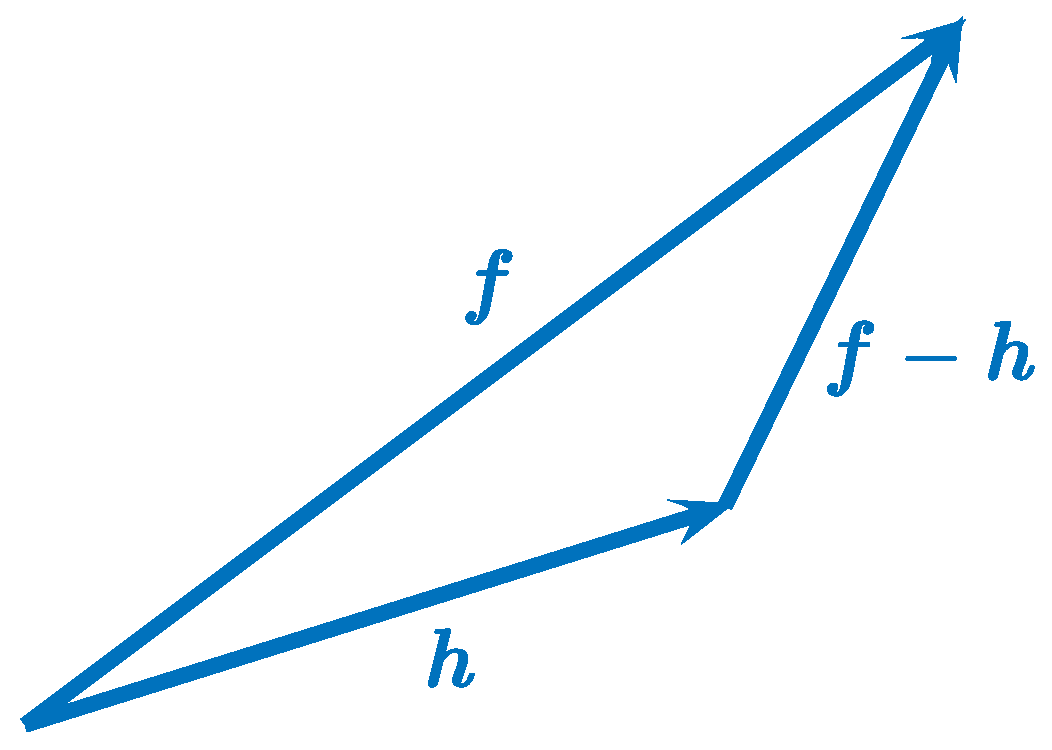
\includegraphics[width=0.5\textwidth]{ProgramsImages/fhfmh.eps}
     \end{center}
\end{column}
\end{columns}

\end{frame}



\begin{frame}[label = generalRiesz]{Riesz Representation Theorem for a Hilbert Space $(V,\ip{\cdot}{\cdot})$}
\begin{theorem}
    If $\LIN: V \to \reals$ is any \alert{continuous} linear real-valued function on the Hilbert space $(V,\ip{\cdot}{\cdot})$, then there \alert{exists a unique} $g \in V$, dependent on $\LIN$, for which $\LIN(f) =  \ip{g}{f}$ for all $f \in V$.
\end{theorem}
\only<1>{
\vspace{-5ex}
\begin{align*}
    \ip{\cdot}{\cdot \cdot} & =  \text{an inner product on } V \times V & \norm{f} & := \sqrt{\ip{f}{f}}\\
    & \qquad \ip{f}{f} > 0 \quad \forall f \ne 0 \\
    & \qquad \ip{f}{h} =\ip{h}{f} \\
    & \qquad \ip{cf+h}{k} = c \ip{f}{k} + c\ip{h}{k} \\
    V & = \text{Hilbert space $=$ a vector space that is \alert{complete} under } \norm{\cdot}  \\
    & \qquad \text{(sequences that should converge  do)} \\
    & \qquad \text{may be \alert{infinite} dimensional $=$ no finite basis}
\end{align*}

Can we prove it \alert{without referring to a basis} for $V$?}
\only<2->{\begin{proof}
\alert{Existence.} \uncover<2-4>{Define $\ker(L) = \{f \in V : \LIN(f) = 0\}$ as the subset of $V$ that $L$ maps into $0$. \only<2>{If $\ker(L) = V$, then all vectors in $V$ are mapped to $0$ and $g = 0$.}\only<3->{$\ker(L) = V$ easy.}} 

\only<3->{Otherwise, pick any nonzero $g_\perp \in \{ h \in V : \ip{h}{f} = 0 \ \forall f \in \ker(L)\}$ \hyperlink{lemma}{\beamergotobutton{How?}}, i.e., $g_\perp$ is orthogonal to all vectors in $\ker(L)$. 
\only<5>{
}  
\only<2-4>{For any $f \in V$, let $h = \LIN(f) g_\perp - \LIN(g_\perp)f$, and note that 
\[
\LIN(h) = L\bigl(\LIN(f) g_\perp - \LIN(g_\perp)f \bigr) = \LIN(f)\LIN(g_\perp) - \LIN(g_\perp)\LIN(f) = 0, \qquad \text{so } h \in \ker(L).
\]
The choice of $g_\perp$ implies that
\[
0 = \ip{g_\perp}{h} = \LIN(f)\ip{g_\perp}{g_\perp}  - \LIN(g_\perp) \ip{g_\perp}{f}, \quad \text{so } \LIN(f) = \frac{\LIN(g_\perp)\ip{g_\perp}{f}}{\ip{g_\perp}{g_\perp}} = \ip{g}{f} \text{ for } g:= \frac{\LIN(g_\perp)g_\perp}{\norm{g}^2}.
\]

\uncover<4->{\alert{Uniqueness.} Same proof as before.}}}
\end{proof}}
    
\end{frame}

\begin{frame}[label = lemma]{There Exists a Nonzero $g_\perp$ Orthogonal to All of $\ker(V)$ \hyperlink{generalRiesz}{\beamerreturnbutton{Back}}}
\begin{lemma}
     If $\LIN: V \to \reals$ is any \alert{continuous} linear functional on the Hilbert space $(V,\ip{\cdot}{\cdot})$, and $\ker(L) := L^{-1}(\{0\}) = \{f \in V : \LIN(f) = 0\} \ne V$,
 	then $ \{ h \in V : \ip{h}{f} = 0 \ \forall f \in \ker(L)\} \alert{\ne \{0\}}$.
\end{lemma}
\begin{proof}
Define $\dist\bigl(h,\ker(L)\bigr) := \inf\{ \norm{h - f} : f \in \ker(L)\}$, i.e., the closest $\ker(L)$ comes to $h$.  For any $h \notin \ker(L)$, choose $k_n \in \ker(L)$ such that $\norm{h - k_n}^2 \le \dist^2\bigl(h,\ker(L)\bigr) + 1/n$ for $n = 1, 2, \ldots$.  By the \alert{parallelogram law}, 
\begin{align*}
	\norm{k_m - k_n}^2 &= \norm{(k_m - h) - (k_n-h) }^2 = 2\norm{k_m - h}^2 + 2\norm{k_n-h}^2 - \norm{(k_m - h) + (k_n-h) }^2 \\
	&= 2\norm{k_m - h}^2 + 2\norm{k_n-h}^2 - 4\norm{(k_m+k_n)/2-h) }^2 \qquad \text{(note that $(k_m+k_n)/2 \in \ker(L)$)}\\
	& \le 2\bigl[\dist^2\bigl(h,\ker(L)\bigr) + 1/m] + 2\bigl[\dist^2\bigl(h,\ker(L)\bigr) + 1/n] - 4\dist^2\bigl(h,\ker(L)\bigr) = 2(1/m+1/n)
\end{align*}
So, $k_n \to k \in V$ due to completeness of $V$; $k \in \ker(K)$ due to continuity of $L$. Let $g_\perp = h - k$.  Then 
\end{proof}
\end{frame}

\end{document}



\finalthanksnote{These slides are  available at \\  \href{https://speakerdeck.com/fjhickernell/quasi-monte-carlo-software}{\nolinkurl{speakerdeck.com/fjhickernell/quasi-monte-carlo-software}}\\
Google Colaboratory notebook at \href{https://tinyurl.com/QMCPyTutorial}{\nolinkurl{tinyurl.com/QMCPyTutorial}}\\
Blog at \href{https://qmcpy.wordpress.com/}{\nolinkurl{qmcpy.wordpress.com/}}}


\thankyouframe


\end{document}




\begin{frame}{Riesz Representation Theorem for $\reals^d$, Alternative Proof}
\begin{theorem}
    If $\LIN: \reals^d \to \reals$ is any linear functional, and $\ip{\vf}{\vh} : = \vf^T \vh$, then there exists a unique $\vg \in \reals^d$, dependent on $\LIN$, for which $\LIN(\vf) =  \ip{\vg}{\vf}$ for all $\vf \in \reals^d$
\end{theorem}
\begin{proof}
\alert{Existence.} Let $\mK$ be the $d$-dimensional identity matrix and let $\vK_j \in \reals^d$ denote its $j^{\text{th}}$ column.  Note that 
\[
f_j = \ip{\vK_j}{\vf} \qquad \forall \vf \in \reals^d.
\]
Now define $\vg \in \reals^d$ by $g_j = \LIN(\vK_j)$.
Then for all $\vf = (f_1, \ldots, f_d)^T$,
    \begin{align*}
    \LIN(\vf) &= L\bigl( \ve_1 f_1 + \cdots + \ve_d f_d \bigr)  = \LIN(\ve_1) f_1 + \cdots + \LIN(\ve_d) f_d \qquad \text{by linearlity} \\
    & = \ip{\vg}{\vf}, \qquad \text{where } \vg = \bigl( \LIN(\ve_1), \ldots, \LIN(\ve_d) \bigr)^T
    \end{align*}
\alert{Uniqueness.} If $\LIN(\vf) =  \ip{\vg}{\vf} =  \ip{\tvg}{\vf}$ for all $\vf \in \reals^d$, then 
\[
0 = \LIN(\vg - \tvg) - \LIN(\vg - \tvg)= \ip{\vg}{\vg - \tvg} - \ip{\tvg}{\vg - \tvg} = \ip{\vg - \tvg}{\vg - \tvg} = \norm{\vg - \tvg}^2
\]
so $\vg - \tvg = \vzero$ and $\vg = \tvg$.
\end{proof}
    
\end{frame}

